% 页数安排:10 10 15 20 20 3 + 15(prefix) + 10(suffix) = 103
% 基于Web-Service的开放式陆地生态系统碳循环模型对比系统构建方法研究
% 开放式陆地生态系统碳循环模型对比系统构建方法研究
\chapter{绪论}

\section{研究背景及意义}

\subsection{研究背景}
% - 介绍全球变化、气候变暖现象,为解决该现象出现的地球系统模式(气候系统模式),陆地生态系统碳循环模型在其中扮演的角色
% - 介绍陆地生态系统碳循环模型的概念、发展、研究现状、对比
% - (碳)模型对比——热点和难点
% - 介绍新兴技术及对碳循环模型对比的意义
% - 总结开放式对比的热点、难点、意义

自工业革命以来,人类活动正在大规模地改变陆地生物圈结构,其中最典型的是温室气体浓度尤其是CO2浓度增加导致的全球气候变暖~\cite{houghton2001climate}。据预测,如果温室气体以目前的排放速率持续下去,地表温度将可能每10年上升0.2℃,100年后的全球平均温度将大约增加2℃(变异范围为1.4\textasciitilde5.8℃)~\cite{Oliver2013Intergovernmental}~\cite{宋燕燕2006陆地碳循环模型的比较分析},由此将会进一步引发一系列严重的全球问题,对人类的发展和社会经济的持续发展带来巨大的威胁。

为了合理预测气候变化特别是全球变暖对生态系统造成的影响,必须深入研究地球系统碳循环过程。而碳循环模型是模拟生态系统,估计和预测不同尺度碳收支格局和变化的重要手段~\cite{cao2003interannual}。从碳循环的完整流程上来看,地球(气候)系统模式包括了碳在海洋、大气、化石、陆地等生态系统中的完整循环流程,是模拟碳循环过程的有效工具。而其中陆地生态系统作为人类活动的聚集地,是四大碳库中最为活跃的一个碳库。陆地生态系统碳循环模型通过对光合作用、呼吸作用、土壤呼吸等过程的对碳循环进行模拟,对植被生产力的模拟和耦合气候模式评估气候变化具有重要作用。

% 以陆地生态系统碳循环领域为例,为了模拟生态系统中大气、海洋、陆表和化石燃料四个碳库之间的碳循环过程,预测不同尺度的碳收支格局和变化情况(Cao M K et al., 2005;Cao,et al.,2003),大气学家研发了众多的碳循环模型,大致可以分为统计模型、遥感参数模型、生态过程模型和遥感、过程耦合模型四类。代表性的有Miami模型~\cite{Lieth1975Primary}、CASA~\cite{Potter1999Interannual}~\cite{Potter2003Continental}、GLO-PEM~\cite{Prince1995Global}~\cite{Goetz2000Interannual}、BIOME-BGC~\cite{running1988general}~\cite{Running1991FOREST}~\cite{thornton2000user}、IBIS(Foley et al., 1996)、LPJ DGVM~\cite{Gerten2004Terrestrial}~\cite{Sitch2010Evaluation}等。各个模型由于其模拟机理不同,有其各自适用的尺度和范围。

陆地生态系统碳循环模型从上世纪90年代以统计模型为代表的兴起,到如今已经经历了长足的发展,从类别上可大致分为统计模型、遥感参数模型、生态过程模型和遥感过程耦合模型。然而,由于碳循环模型涉及到的生物、物理、化学和地球机理的复杂性,各个模型有其各自的适用时空尺度的先决条件,在应用时往往难以进行选择,其模拟结果也不尽相同。为了评估气候模型的适用情景、模拟效果、参数敏感性和气候的历史规律及未来趋势,世界气候研究计划(WCAR,World Climate Research Programme)组织了6次耦合模型对比计划(CMIP,Coupled Model Intercomparison Project),针对每届IPCC(IPCC,Intergovernmental Panel on Climate Change)评估报告中出现的科学问题制定标准实验方案,对比各个模型的模拟能力~\cite{meehl2000coupled}。其中,目前正在开展的第六阶段耦合模型对比计划(CMIP6)背书的模型对比项目有23余个,包括气溶胶和化学模型对比项目、耦合气候碳循环模型对比项目、云反馈模型对比项目、十年际气候预测项目、海洋模型对比项目、古气候模型对比项目、辐射强迫模型对比项目等~\cite{eyring2016overview}~\cite{WCRP-CMIP6-Endorsed-CMIPs}。除此此外,区域气候模型评估系统(RCMES,Regional Climate Model Evaluation System)和协调区域气候降尺度实验(CORDEX,Coordinated Reginal Climate Downscaling Experiment)也在区域尺度上开展气候模型的对比评估,通过区域尺度上的评估决策弥合全球尺度上的气候变化~\cite{loikith2013scientific}。在陆地碳循环领域,全球分析、集成和建模(GAIM, Global Analysis, Integration, and Modelling)工作组和生态系统模型数据对比计划对植被净第一性生产力(NPP,Net Primary Productivity)进行了对比。
可见,模型对比评价是当前碳循环研究领域的一个\textbf{热点}。但是,现有的对比计划大多数都是针对气候系统模式模拟的地球系统碳循环,针对陆地生态系统碳循环模型的对比还相对较少。

据统计,在第五次耦合模型比较计划(CMIP5)中,超过20个建模组使用50多个碳循环模型参与模拟~\cite{Taylor2012An};在GAIM对比项目中,超过15个陆地碳循环模型参与对比~\cite{cramer1999comparing}~\cite{kicklighter1999comparing},
越来越多的模型参与到对比计划中。但是,模型对比仍然面临着诸多困难:

\begin{enumerate}[(1)]
    \item \textbf{从碳循环的过程上来看},碳循环模型通常涉及到生物(光合作用、呼吸作用)、物理(植被冠层能量交换)、化学(碳、水循环)、遥感(数据同化)等模块,每个模型由于其机理不同,涉及到的模块组成往往不同,而且各个模块的实现方法也不尽相同;
    \item \textbf{从模型开发视角上来看},碳循环模型由不同的科研人员编写,面临着操作系统、编程语言、软硬件环境依赖、运行方式、输入输出数据格式等多方面的异构性,难以部署、编译和应用,阻碍了模型的推广;
    \item \textbf{从数据搜集上来看},不同的碳循环模型需要的驱动数据不尽相同,在模型对比时需要在数据搜集和预处理上耗费巨大的精力;
    \item \textbf{从模型对比的层面上来看},碳循环模型的对比应该从多个层面上开展,包括单个观测站点层面、不同植被功能类型的差异性和全球范围的时空分布格局等。
\end{enumerate}

这些原因共同限制了模型对比工作的发展,模型对比也是当前碳循环模型研究领域的一个\textbf{难点}。

随着计算机和网络技术的发展,Web Service和面向服务的软件架构(SOA,Service-Oriented Architecture)技术不断成熟,地理模型和数据逐渐朝着网络服务化的方向进行封装与共享~\cite{adgeo-4-69-2005}~\cite{peckham2009componentizing}~\cite{胡迪2015地理模型的服务化封装方法研究},为碳循环模型对比过程中面临的难点提供了技术上的有效支撑。服务化的地理模型将复杂的地理模型封装为一个黑箱,屏蔽了模型在机理上和操作上的复杂性和异构性,大大降低了碳循环模型的应用难度~\cite{胡迪2015地理模型的服务化封装方法研究}~\cite{yue2016service};地理数据服务不仅可以降低数据搜集的困难,更重要的是解决了网络环境下数据与模型难以互操作的问题~\cite{Yue2015A}。
\textbf{本文基于微服务的分布式网络架构,设计了一套高效稳定可用的陆地生态系统碳循环模型对比框架,开放了一系列模型资源、数据资源和对比资源服务化接入接口,通过科学工作流驱动模型服务、数据服务和对比服务的集成互操作,实现了陆地生态系统碳循环模型的对比。}

\subsection{研究意义}
% - 通用的意义:开放、公平、可共享、可重用。
% - 对碳循环模型的意义:促进碳循环模型的发展改进,提高碳循环模型的精度,提高人们对碳排放的认知,为解决气候问题提供准确有效的模拟手段。

本文基于网络服务开展模型的对比,通过模型资源、数据资源和对比方法及方案的服务化封装、部署、发布、共享和集成,为陆地生态系统碳循环的对比提供了一种新的方案。对于陆地生态系统碳循环模型来说,屏蔽了彼此之间的异构性和复杂性,实现了模型资源的共享,促进了模型的应用推广和发展;对比碳循环相关数据来说,降低了数据收集、存储、管理、处理的繁琐流程;对于模型对比来说,一方面可以将传统的线下对比过程公开化、透明化,使对比过程具有可追溯性、可验证性和易重复性,另一方面对比方案也可以共享出来,在研究不同时空尺度的地区时,可以重用起来。

\section{国内外研究现状综述}
开放式陆地生态系统碳循环模型对比系统的构建涉及多个方面,包括模型和数据资源的深入了解、模型对比评价方法的总结归纳、以及开放式服务化系统架构的搭建。认识地理模型的运行行为特征和数据特征是驱动其模拟计算的前提,剖析前人对比领域模型的统计学方法是丰富对比形式的手段,熟悉开放式服务化系统的框架是构建系统的基础。因此,本文从陆地生态系统碳循环模型的发展历程,前人对碳循环模型的对比评价方法以及开放式服务化系统的框架三个方面进行回顾,分析陆地生态系统碳循环领域地理模型对比的研究现状、存在问题和发展趋势。

\subsection{陆地生态系统碳循环模型}
% 模型机理介绍

陆地、大气、海洋以及化石燃料碳库是地球系统碳循环的四个主要组成部分,其中陆地生态系统又是其中最为活跃的碳库,也是人类活动聚集的场所。陆地生态系统碳循环模型通过模拟植物光合器官碳库、植物支持器官碳库、凋落物碳库和土壤有机碳库之间的碳源汇交换,来计算植被的初级生产力~\cite{毛留喜2006陆地生态系统碳循环模型研究概述}。

陆地生态系统碳循环模型从机理上可分为统计模型、生态过程模型和遥感、过程耦合模型。统计模型可分为气候统计模型和遥感统计模型。其中气候统计模型主要通过在气候因子与植被净初级生产力(Net Primary Productivity,NPP)的实测数据之间建立回归方程;遥感统计模型通过遥感光谱指数(如NDVI)与NPP、生物量等数据间的相关关系进行统计回归。统计模型简单直观,具有较强的区域适用性,但其完全依赖于地面观测数据,对于不同的区域,模型不具备普适性和推广性。同时统计模型没有考虑陆地生态系统碳循环过程的内部机理,无法揭示生态系统与环境间的相互影响关系,不能用于对未来的预测研究~\cite{袁文平2014陆地生态系统植被生产力遥感模型研究进展}~\cite{谢馨瑶2018大尺度森林碳循环过程模拟模型综述}。生态过程模型按照是否考虑实际环境对植被类型、组成和结构的影响分为基于动态植被类型的模型和基于静态植被类型的模型~\cite{王绍刚2008森林碳循环模型方法研究进展}~\cite{王萍2009森林碳循环模型概述}~\cite{毛留喜2006陆地生态系统碳循环模型研究概述},按照涉及到的机理类型分为地球化学过程模型、陆面物理过程模型和生物过程模型~\cite{谢馨瑶2018大尺度森林碳循环过程模拟模型综述}。过程模型由于其综合考虑了碳循环过程的动力学特征,结合了气候、土壤和植被生理生态参数,以及陆地生态系统与大气、海洋之间的相互作用,模拟结果相对来说更加准确,逐渐占据了主导地位。遥感、过程耦合模型通过将遥感观测数据(如叶面积指数LAI)同化到模型之中,来提高模型模拟的精度~\cite{2013基于数据同化的哈佛森林地区水、碳通量模拟},他融合了遥感统计模型和生态过程模型的优点,可以反映区域和全球尺度的NPP空间分布和变化~\cite{朱文泉2005陆地植被净初级生产力计算模型研究进展}。

综上所述,生态过程模型在全球范围内不仅模拟效果好,而且与遥感、过程耦合模型相比更加简单、容易实现。因此,本文选取了三个适合全球尺度的生态过程模型参与对比:IBIS、BIOME-BGC、LPJ DGVM,并总结了各自的特征,如表1所示。从中可知,这些模型的时空适用范围、输入数据、输出要素都很相似,均具备全球范围内碳循环的模拟能力,彼此之间可以进行对比。


\subsection{碳循环模型的验证与对比}
对于陆地生态系统碳循环模型模拟结果的验证和对比,前人大多从多个视角进行综合对比,包括对模拟结果的可视化观察对比,使用统计学方法定量地对比等。没有单独的评价手段被认为是优越的,相反的,多种对比技术的结合使用能够为模型模拟能力提供全面评价~\cite{Taylor2012An}。

在对比对象方面,目前主要分为三类:基于通量站点数据的对比、基于卫星遥感数据的对比和基于多模型模拟结果的交叉对比。杨延征~\cite{杨延征2016基于}、王磊(2010)、刘曦~\cite{刘曦2011IBIS}、张海燕(2006)等人分别在中国全国尺度、中国东部、东北东部森林和东北帽儿山应用IBIS模型估算碳排放情况,将模型模拟的结果与通量站点观测数据对比,验证其在中国的模拟能力。胡瀞予(2011)、NIU Ben~\cite{Niu2017Satellite}等人分别以台湾陆域生态区和青藏高原为研究区域,将生物测定法、Rahman’s方程式以及VPM、PCM、AVM的模拟结果与MOD17数据集相对比,评估其模拟能力。P.Friedlingstein(2006)在CMIP4中通过11个碳循环模型之间模拟结果的相互比较来评价其模拟能力。

在对比方法方面,通过绘制模拟值等值线图、观测值等值线图、差异等值线图可以非常直观地展示出各个模型模拟结果的差异;通过泰勒图展示模拟值与观测值之间的标准差之比、均方根误差以及相关系数;通过纵向图和时间序列折线图可以清晰地展现模型在各个子区域中的适用情况~\cite{Kim2013Evaluation}~\cite{Kim2014Evaluation}~\cite{Kim2017Winter}~\cite{刘敏200913}(Kim J,2012;Kim J,2014;Kim J,2018;郭彦,2013;刘敏,2009)。Stoner A M K~\cite{Stoner2013An}使用统计降尺度的方法建立当前观察值、当前模拟值、未来模拟值与未来观察值之间的关系,预测未来的气候因子发展状态。

在对比框架方面,国际上比较知名的是WCAR开展的CMIP。通过制定一系列证明模型模拟能力的标准实验,参与比较的模型都遵循实验协议进行测试。使用一致的预测因子(如数据源、空间分辨率、时间分辨率等),针对特定的预测指标(如温度、湿度、降水量、NPP等),在一致的时间范围内模拟,最后将模拟结果提交给专家评审,通过审核的对比结果被公开发布在网站上~\cite{Taylor2012An}。耦合模型对比计划、协调区域降尺度实验以及区域气候模型评估系统都遵循着这种对比框架开展对比~\cite{eyring2016overview}~\cite{Gutowski2009The}~\cite{赵宗慈2016CMIP6}。


\subsection{开放式服务化系统框架}
随着计算机技术的发展,越来越多的数据被发布为服务,其中具有代表性的是开放地理信息联盟(OGC,Open Geospatial Consortium)的WMS、WFS、WCS。在地理模型和数据处理方法方面,OGC WPS(Web Processing Service)也为地理模型的共享提供了解决办法。 %~\cite{Castronova2013Models}

袁爽~\cite{袁爽2010空间数据}基于OGC WFS、WMS标准,实现了空间数据的服务发布;吴楠~\cite{吴楠2012基于}、毛曦~\cite{毛曦2012基于}、宋东泽~\cite{宋东泽2015一个生态传感网的}基于OGC WPS标准,分别设计并实现了VPM模型和日均蒸散量模型的服务发布。Yue S~\cite{Yue2013Key}~\cite{Yue2015A}基于Web Service提出了一套模型服务的元数据描述、封装、打包和发布的技术体系。

\subsection{研究现状分析与总结}
% 存在的问题及展望
纵观陆地生态系统碳循环模型的研究现状,陆地生态系统碳循环模型的理论体系越来越完善,应用越来越广泛。随着IPCC等国际组织的牵头推动,模型的对比和评价也逐渐开始开展,极大地促进了模型的改进和发展。分析当前的研究现状总结为以下几点:

\begin{enumerate}[(1)]
\item \textbf{陆地生态系统碳循环模型:}

随着技术手段的不断成熟,越来越多的模型被开发出来。但由于地球系统的复杂性,模型在类别、机理、模块结构、参数、数据等方面形态各异,这种多样性阻碍了模型在不同区域以及全球范围内的应用推广,开展模型对比是解决该问题的有效技术手段;

\item \textbf{碳循环模型的对比:}

碳循环模型的对比是当前的研究热点和难点,在对比对象方面模型可以与通量观测站点、遥感影响影像数据以及其他模型的模拟结果相对比;在对比方法方面大多数采用可视化方法和统计学手段;在对比框架方面世界气候研究计划制定了一套模型对比的实验方案,参与者通过实验内容的实施、提交、评审,最终可以将对比结果公开出来。目前的对比相对完善,但是在互联网技术的高速发展下,有待进行一些新的技术尝试;

\item \textbf{开放式服务号系统框架:}
% OGS WPS 标准的缺点:
% 数据基于栅格和GML
% 不支持模型集成
服务号包括模型资源的服务化和数据资源的服务化。目前基于OGC的WFS、WMS和WPS标准形成了一套成熟的技术体系。模型服务和数据服务地发布,可以降低模型的使用难度,促进模型的应用和完善,但是这种技术手段在气候模型以及模型的对比方面缺乏广泛地应用。
\end{enumerate}

\section{研究目标与研究内容}

\subsection{研究目标}
针对目前地理模型和数据资源分散、模型安装部署困难、模型模拟效果难以评估、评估成果难以再现的问题,本文以陆地生态系统碳循环模型为例,基于Web Services技术,旨在设计并实现一个提供模型对比的“擂台”,并用IBIS、BIOME-BGC和LPJ三个模型验证平台的实用性。具体研究目标包括:
(1)	设计出一套新的基于网络服务的开放式地理模型对比系统框架;
(2)	以陆地生态系统碳循环模型为例,实现地理模型资源和数据资源的开放式接入; 
(3)	以陆地生态系统碳循环模型为例,实现对比方案的构建和实施。


\subsection{研究内容}
为实现上述研究目标,设计研究内容如下:
\begin{enumerate}[(1)]
    % 陆地生态系统碳循环模型的分析和应用
    % 陆地生态系统碳循环模型的开放式对比框架设计
    % IBIS、Biome-BGC、LPJ三个模型对植被生产力模拟的对比
\item \textbf{开放式地理模型对比系统框架的构建}

开放式对比系统框架是开展详细对比工作的基础支撑,它描述了模型资源、数据资源、对比方法资源的标准接入方式,所有这些资源在框架的规范下以科学工作流的方式,有条不紊地运行、耦合、集成。

考虑到网络资源的传输成本、模型运算和模型对比的业务逻辑,本文将整体服务器框架分为三部分:1)资源服务器:负责数据存储、数据库管理、数据服务发布和数据缓存;2)模型计算服务器:负责模型服务发布、模型调用、数据处理和分布式计算;3)模型对比服务器:负责资源汇总和展示、对比方案的构建、对比任务的分发和比较结果的可视化。三个部分之间通过Http和Ftp协议通信。这种情况下,地理模型、地理数据、数据处理方法、数据可视化方法和数据对比方法都以组件的形式分别插入到各个模块中,实现了系统架构的解耦。

\item \textbf{开放式地理模型资源的接入}

地理模型资源是参与模型对比的主体,通过模型资源的汇聚形成模型资源库,而模型资源库是模型对比的重要组成部分。为了实现模型资源的开放式接入,首先需要定义一套模型的元数据描述接口,其中包括模型的属性描述、模型的调用接口描述和模型的软硬件依赖环境描述,结合Web Service技术,通过应用服务器向外暴露Restful API可以将地理模型发布为服务,模型服务向数据库中注册可以实现模型服务的管理。在本文中发布的模型条目包括IBIS、BIOME-BGC、LPJ DGVM。

\item \textbf{开放式地理数据资源的接入}

地理数据资源的接入是驱动模型运行的基础。对于地理数据资源的接入方法和模型资源类似。对于本文涉及到的碳循环模型的运行,需要发布的数据服务包括陆面掩膜数据、气象数据、土壤数据、植被数据和其他配置数据。其中气象数据的时间分辨率是1天,气象参数包括最高温、最低温、日均温、降水量、相对湿度、平均风速、大气压和云覆盖率等;土壤数据包括沙粒含量和黏土含量等;植被数据包括植被类型、凋落物储量和植被功能型数据等。

\item \textbf{地理模型对比方案的构建和实施}

由于单一的对比方法不能够完备地展示出各个模型之间的差异,本文的对比从构建对比方案入手。对比方案是从多个视角综合对比几个模型的模拟能力,是多个对比方法的组合。因此,在构建对比方案之前,首先要构建一个对比方法库,包括现阶段流行的偏差等值线图、泰勒图、时间序列折线图、纵向图、区域降尺度等统计学方法都作为对比方法库的成员,每种对比方法针对特定的结果数据集作出评价。最后,对比方案通过配置具体的输入数据开始模拟,模拟结束会生成一个评价报告文档。在这个过程中,对比方案也作为一种开放的资源共享和重用起来。
\end{enumerate}


\section{研究方法与技术路线}

\subsection{研究方法}
\begin{enumerate}[(1)]
\item \textbf{文献分析法}

搜集并整理国内外相关领域研究者关于陆地生态系统碳循环模型、模型对比方法、模型和数据共享与服务化方法的研究成果,总结前人研究方法的特点和使用范围,针对这些成果的优劣势进行分析和借鉴,为本文的研究方法提供思路。

\item \textbf{归纳演绎法}

分析地理模型在运行行为上的特征,对比并归纳其调用方式,在此基础上设计模型的元数据描述接口,为模型的服务化方法做准备。

\item \textbf{数理统计法}

本文对模型模拟结果的对比评价分析是通过在模型模拟结果与实测值之间进行统计分析,根据统计特征值来评价模拟结果的优劣。

\item \textbf{案例验证法}

本文以IBIS、BIOME-BGC、LPJ模型为例,对各个模型进行封装,以满足模型在站点和区域上的模拟计算,并对模拟结果进行数理统计,分析其优缺点。
\end{enumerate}


\subsection{技术路线}
根据本文的研究目标和研究内容,本文设置的技术路线如~\ref{fig:tec-route}所示,包括5个阶段:1)问题分析与资料整理阶段。收集并整理文献,分析现有陆地生态系统碳循环模型的特征、碳循 环模型的对比方法和开放式服务化系统架构,确定本文的研究思路;2)模型对比系统框架的构建:搭建系统的整体网络架构,设计各个服务器模块的功能职责和服务器之间的通信方式;3)模型和数据资源的开放式接入:根据模型资源和数据资源的特点,分别设计其开放式资源接入方法;4)模型对比方案的构建和实施:首先丰富模型对比方法库,然后根据模型对比方法的组合和综合评价标准构建模型对比方案,配置数据后调用模型生成评价对比报告;5)实验验证:根据选取的三个模型分别在全球陆地范围内进行模拟,对比其模拟水平。

\begin{figure}[!htbp]
    \centering
    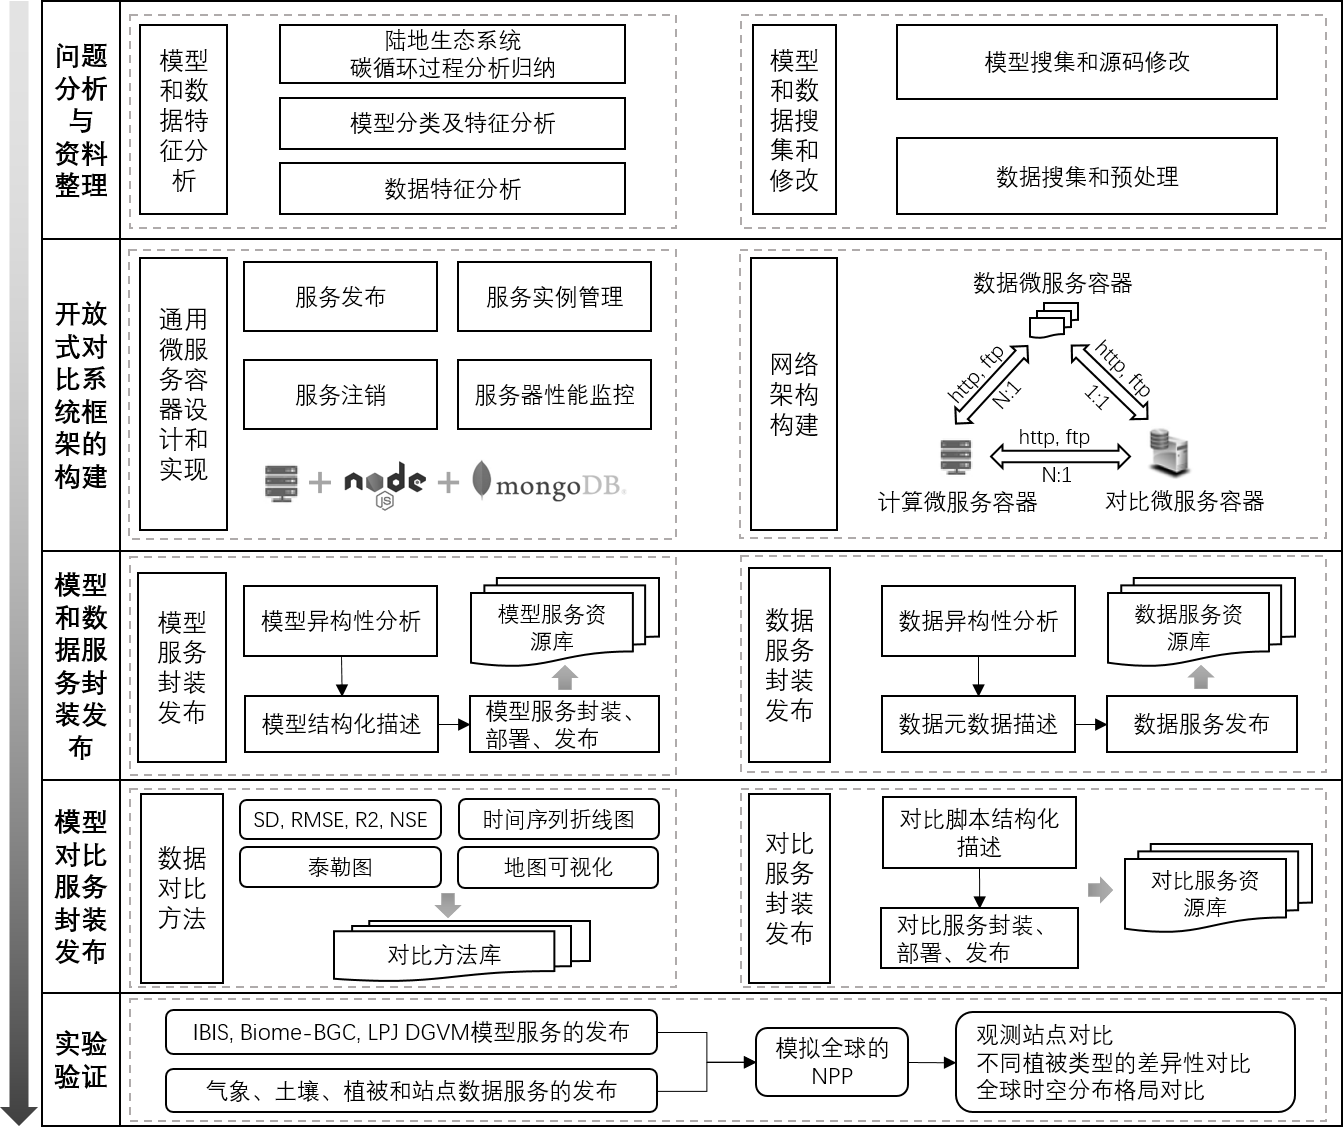
\includegraphics[width=1\textwidth]{tec-route}
    \caption{技术路线}
    \label{fig:tec-route}
\end{figure}

\section{论文组织结构}
第一章:绪论。介绍开放式对比的意义,梳理当前国内外的研究现状,得出模型对比是碳循环领域内的一个热点和难点,并提出了当前时代下开放式服务化技术体系可以为模型对比提供了新的思路,在此基础上确定了本文的研究目标、研究内容、研究方法,并设计了具体的技术路线。

第二章:碳循环、碳循环模型及数据。本章概述地球系统碳循环的基本结构,并确定陆地生态系统碳循环在其中的位置和作用。总结归纳了陆地生态系统碳循环模型的概念、结构、分类体系和优缺点,指出当前的陆地生态系统碳循环模型可分为统计模型、生态过程模型和遥感、过程耦合模型,并详细介绍了参与本文对比的三个生态过程模型模型:IBIS、Biome-BGC、LPJ。最后介绍这三个模型运行所需的数据、通量网的观测数据和遥感通量数据产品。

第三章:陆地生态系统碳循环开放式对比框架。本章从四个角度详细叙述了开放式的对比框架。首先,对国际上的开展的对比计划中所涉及到的对比情景进行分析总结,得出对比情景包括历史情景、未来预测情景、敏感性分析情景和参数校准情景等,在对这些情景的业务执行流程进行抽象归纳后,将对比流程抽象为创建对比话题、对比方案和对比任务的三步,并对系统的功能进行了整体设计;其次,从组件视角上分析了框架下面包含的地理资源组件模块,这些模块包括模型服务资源库、数据服务资源库、单位量纲资源库、数据重构服务资源库、可视化服务资源库和对比服务资源库,并详细介绍了每种组件服务的标准开放接口;再次,从网络架构的视角上选择了微服务的分布式架构,将计算节点分布在n台计算节点、1台资源节点、1台对比节点上,使系统整体功能有效分割同时又不显得过于臃肿;最后,从科学工作流执行流程的视角上,分析总结了对比的流程,并设计自动化执行引擎以驱动模型对比工作。

第四章:开放式对比资源接入方法。本章指出在开放式对比框架下,对比资源的开放式接入方法是系统的关键,并将对比资源分为数据资源、模型资源和对比方法资源三类。因此,本章分三个小节详细介绍三种资源的开放式接入方法。
对于数据资源,首先从格式、尺度和编排四个角度分析本文所用数据的特点,对领域通用标准数据设计结构化描述文档,对非标准数据采用示例数据URL的形式进行描述。然后遵循OGC WMS/WFS/WCS标准,使用GeoServer发布数据服务,并提供数据下载服务和数据处理服务;
对于模型资源,首先针对其特点进行分析,总结模型在参数策略、运行流程上的相同点和在开发层面的异构点。针对这些特征分三个视角进行结构化描述:面向人类理解的基本信息描述;面向机器运行的运行信息描述;面向模型部署的软硬件依赖环境描述。最后设计支持有源代码、无源代码和简单模型、集成模型的封装策略,在此基础上进行模型服务部署和发布。
对于对比资源...

第五章:原型系统和案例验证。

第六章:结论和展望。